% Generated from: Zhihu/专栏：概率与统计/渐近统计 (3) ：中心极限定理_金鱼马_2026-06-09.md
概率和统计的意义在于描述由大量随机因素影响所表现出来的规律性，因此，研究随机变量和的极限对于搞清楚随机现象的本质有着极其重要的价值。这之中最为重要的结论，莫属中心极限定理 (Central Limit Theorem, CLT)。关于这个定理，大家熟悉的形式一般有下面两种。

\begin{theorem}[De Moivre--Laplace 中心极限定理]
设一列随机变量 $\{X_n\}_{n=1}^\infty$ i.i.d. 服从两点分布
\[
P(X_1=1)=p,\qquad P(X_1=0)=1-p,\qquad 0<p<1.
\]
令 $S_n=\sum_{k=1}^nX_k$，那么
\[
\frac{S_n-np}{\sqrt{np(1-p)}}\overset{\rm d}\longrightarrow\mathcal N(0,1),
\qquad n\to\infty.
\]
\end{theorem}

\begin{theorem}[Lindeberg--L\'evy 中心极限定理]
设一列随机变量 $\{X_n\}_{n=1}^\infty$ i.i.d.，总体均值为
$\mathbb E[X_1]=\mu$，方差为 $\operatorname{Var}[X_1]=\sigma^2<\infty$。
令 $S_n=\sum_{k=1}^nX_k$，那么
\[
\frac{S_n-n\mu}{\sqrt n\sigma}\overset{\rm d}\longrightarrow\mathcal N(0,1),
\qquad n\to\infty.
\]
\end{theorem}

历史上，CLT 理论的发展很大程度得益于 20 世纪 20 年代特征函数的引入。前述结论已经在第~\ref{ch:characteristic-functions}~章中用“特征函数 + L\'evy 连续定理”得到证明。

但在实际应用中，我们经常遇到更一般的情况：
\begin{itemize}
\item 每个 $X_i$ 独立但可能具有不同的分布；
\item 每个 $X_i$ 可能不独立，而是存在某种相依性。
\end{itemize}
这就需要我们寻找更一般的极限定理。

此外，除了减弱随机变量的同分布以及独立性要求，CLT 的研究还有两个方向：讨论向标准正态分布 $\mathcal N(0,1)$ 收敛的问题，以及计算估计收敛的速度（Berry--Esseen 界）等。

本章将证明独立不同分布情况下随机变量组列的两个重要极限定理：Lyapunov CLT 和 Lindeberg--Feller CLT；以及非独立的一种情形：$m$-相依随机变量列的中心极限定理。主要参考 Chung~\cite[第 7 章]{chung2001}。

首先，我们讨论极限理论的一般问题。与其讨论随机变量列，我们在此讨论其“组列”：
\[
\begin{array}{cccc}
X_{11},&X_{12},&\cdots,&X_{1k_1},\\
X_{21},&X_{22},&\cdots,&X_{2k_2},\\
\vdots&\vdots&&\vdots\\
X_{n1},&X_{n2},&\cdots,&X_{nk_n},\\
\vdots&\vdots&&\vdots
\end{array}
\]

\begin{definition*}[独立随机变量组列]
对任意 $n\ge1$，设 $\{X_{n1},X_{n2},\dots,X_{nk_n}\}$ 是概率空间
$(\Omega_n,\mathcal F_n,P_n)$ 上的一组随机变量，满足
$X_{n1},\dots,X_{nk_n}$ 相互独立，且当 $n\to\infty$ 时 $k_n\to\infty$。
则 $\{X_{nj}:1\le j\le k_n\}_{n\ge1}$ 被称作独立随机变量的组列，也叫做“双阵列 (double array)”。本章中涉及的组列都满足独立性，不再反复说明。
\end{definition*}

传统的随机变量列 $\{X_n\}_{n=1}^\infty$ 里，每增加一个 $n$，我们只是在原始序列中多取一个随机变量；这隐含地假定了随机变量的分布是“固定”的：随着 $n$ 增大，我们只是累积更多的样本。然而在组列 $\{X_{nj}:1\le j\le k_n\}_{n\ge1}$ 里，每一行的随机变量个数、分布可以完全不同，因而也更加灵活。传统随机变量列只是组列的一个特例，它可以视作三角组列 $\{X_j:1\le j\le n\}_{n\ge1}$。

我们讨论的目标是形如 $S_n:=\sum_{j=1}^{k_n}X_{nj}$ 的行和，当 $n\to\infty$ 时的极限是什么？收敛于极限分布族中某一给定分布的条件是怎样的？

这里约定符号
\[
\begin{aligned}
\mu_{nj}&:=\mathbb E[X_{nj}],
&\mu_n&:=\sum_{j=1}^{k_n}\mathbb E[X_{nj}]=\sum_{j=1}^{k_n}\mu_{nj},\\
\sigma_{nj}^2&:=\operatorname{Var}[X_{nj}],
&\sigma_n^2&:=\sum_{j=1}^{k_n}\operatorname{Var}[X_{nj}]=\sum_{j=1}^{k_n}\sigma_{nj}^2.
\end{aligned}
\]
在使用这些符号时总假定其为有限值。

\section{Lyapunov 中心极限定理}

\subsection{Lyapunov 条件和 Lyapunov CLT}

\begin{theorem}[Lyapunov CLT]

\label{thm:ch3:3-1}

对独立随机变量组列$\{X_{nj} : 1 \leq j \leq k_n\}_{n \geq 1}$，记 $\Gamma_n := \sum_{j=1}^{k_n} \mathbb{E}\big[|X_{nj} - \mu_{nj}|^3\big]$，且该值对每个 $n$ 都是有限的。那么，若下述的 \textbf{\emph{Lyapunov 条件 }} 成立：
\[\frac{\Gamma_n}{\sigma_n^3} = \frac{1}{\sigma_n^3} \sum_{j=1}^{k_n} \mathbb{E}\big[|X_{nj} - \mu_{nj}|^3\big] \to 0 \quad \text{当 } n \to \infty\]
则
\[
\frac{S_n - \mu_n}{\sigma_n} \overset{\rm d}\to\mathcal N(0, 1).
\]

\end{theorem}

\begin{remark}
定理中的 3 阶矩条件其实过强，常数 3 可以换作任意的 $2+\delta$，其中 $\delta>0$。这种情况下的证明也完全类似。
\end{remark}

容易看到，随机变量列 $\{X_j\}_{j=1}^\infty$ 的 CLT 是定理~\ref{thm:ch3:3-1} 的直接推论，或者更直白地，定理~\ref{thm:ch3:3-1} 能直接翻译成随机变量列的形式：设 $\{X_j\}_{j=1}^\infty$ 是一列独立的随机变量，且对诸 $j$ 有 $\mathbb{E}[X_j]=\mu_j$ 、 $\mathrm{Var}[X_j]=\sigma_j^2<\infty$ 、 $\mathbb{E}[|X_j-\mu_j|^3]=\gamma_j<\infty$ 。若下述 Lyapunov 条件成立：
\[
\frac1{\sigma_n^3}\sum_{j=1}^n\gamma_j\to 0,\quad \text{当 } n \to \infty,
\]

那么
\[
\frac{S_n - \mu_n}{\sigma_n} \overset{\rm d}\to \mathcal{N}(0, 1).
\]

Lyapunov CLT 的一个直接推论如下。

\begin{corollary}

\label{cor:ch3:3-2}对独立随机变量组列$\{X_{nj} : 1 \leq j \leq k_n\}_{n \geq 1}$，若 $\left|\frac{X_{nj}}{\sigma_{n}}\right|\le M_{nj}$ a.s.，且 $\lim\limits_{n\to\infty}\max_{1\le j\le k_n}M_{nj}=0$，那么
\[
\frac{S_n-\mu_n}{\sigma_n}\overset{\rm d}\longrightarrow\mathcal N(0,1).
\]

\end{corollary}

\begin{proof}

注意到 $\mathbb{E}[|X_{nj}-\mathbb{E}[X_{nj}]|^3]\le 2M_{nj}\sigma_n\mathbb{E}[|X_{nj}-\mathbb{E}[X_{nj}]|^2]=2M_{nj}\sigma_n\sigma_{nj}^2$ ，因此 \[ \sum_{j=1}^{k_n}\mathbb{E}\big[|X_{nj}-\mathbb{E}[X_{nj}]|^3\big]\le 2\sigma_n\left(\max_{1\le j\le k_n}M_{nj}\right)\sum_{j=1}^{k_n}\sigma_{nj}^2=2\sigma_n^3\max_{1\le j\le k_n}M_{nj} \]故 $\max\limits_{1\le j\le k_n}M_{nj}\to 0$ 成立蕴含 Lyapunov 条件成立。

\end{proof}

该推论会在后文中用于 Lindeberg-Feller CLT 的证明。

接下来我们将使用两种方式证明定理~\ref{thm:ch3:3-1}。

\subsection{准备工作一}

我们知道，与实数情况类似，当复数 $|z|<1$ 时有``Taylor 展开''
\[\log(1+z) = \sum_{n=1}^{\infty} (-1)^{n-1} \frac{z^n}{n}\]
这里 $\log$ 是复对数函数主支。

下面的引理可以视作重要极限 $\lim\limits_{n \to \infty} \left(1 + \tfrac\theta n\right)^n \to e^\theta$ 的推广，在后面能帮助我们``将复杂的乘积转化为相对简单的形式''。

\begin{lemma}

\label{lem:ch3:3-3}

令 $\{ \theta_{nj} : 1 \leq j \leq k_n \}_{n \geq 1}$ 是一个复数的组列，满足当 $n \to \infty$ 时：

\begin{enumerate}
\def\labelenumi{\arabic{enumi}.}
\tightlist
\item
  $\max\limits_{1 \leq j \leq k_n} |\theta_{nj}| \to 0$，
\item
  $\sum\limits_{j=1}^{k_n} |\theta_{nj}| \leq M < \infty$，其中 $M$ 与 $n$ 无关，
\item
  $\sum\limits_{j=1}^{k_n} \theta_{nj} \to \theta$，其中 $\theta$ 是一个有限复数，
\end{enumerate}

则
\[
\prod_{j=1}^{k_n}(1+\theta_{nj})\to e^\theta.
\]

\end{lemma}

\begin{proof}

条件 (1.) 意味着当 $n$ 充分大时有
\[
\max_{1\le j\le k_n}|\theta_{nj}|\le \frac12.
\]
因此，对每个 $j\le k_n$，复数 $1+\theta_{nj}$ 都位于圆盘 $D(1,1/2)$ 内。该圆盘包含于右半平面，既不包含原点，也不与复对数主支的分支切线相交，故可以统一使用上述 Taylor 展开。此时
\[
\begin{aligned}
\left|\log(1+\theta_{nj})-\theta_{nj}\right|
&=\left|\sum_{m\ge2}(-1)^{m-1}\frac{\theta_{nj}^m}{m}\right|\\
&\le \sum_{m\ge2}\frac{|\theta_{nj}|^m}{m}\\
&\le \frac{|\theta_{nj}|^2}{2}
  \sum_{m=2}^{\infty}\left(\frac12\right)^{m-2}\\
&=|\theta_{nj}|^2.
\end{aligned}
\]
当 $\theta_{nj}\ne0$ 时，令
\[
\lambda_{nj}
:=\frac{\log(1+\theta_{nj})-\theta_{nj}}{|\theta_{nj}|^2};
\]
当 $\theta_{nj}=0$ 时，令 $\lambda_{nj}=0$。于是 $|\lambda_{nj}|\le1$，并且
\[
\log(1+\theta_{nj})
=\theta_{nj}+\lambda_{nj}|\theta_{nj}|^2.
\]
因此
\[
\sum_{j=1}^{k_n}\log(1+\theta_{nj})
=\sum_{j=1}^{k_n}\theta_{nj}
+\sum_{j=1}^{k_n}\lambda_{nj}|\theta_{nj}|^2.
\]
\begin{itemize}
\tightlist
\item
  根据条件 (3.)，上式右侧第一项趋于 $\theta$ 。
\item
  根据条件 (1.) 和 (2.)，上式右侧第二项趋于 0，
\end{itemize}
\[\left|\sum_{j = 1}^{k_n}\lambda_{n j}|\theta_{n j}|^{2}\right|\leq \max_{1\leq j\leq k_{n}}|\theta_{n j}|\sum_{j = 1}^{k_{n}}|\theta_{n j}| \leq \max_{1\leq j\leq k_{n}}|\theta_{n j}|M \to 0\]
这就证明了
\[
\sum_{j=1}^{k_n}\log(1+\theta_{nj})\to\theta.
\]
最后，注意这里并不需要使用复对数通常不成立的乘法公式。直接利用指数函数，有
\[
\begin{aligned}
\prod_{j=1}^{k_n}(1+\theta_{nj})
&=\prod_{j=1}^{k_n}\exp\!\bigl(\log(1+\theta_{nj})\bigr)\\
&=\exp\!\left(\sum_{j=1}^{k_n}\log(1+\theta_{nj})\right)
\longrightarrow e^\theta.
\end{aligned}
\]
这便证明了结论。

\end{proof}

第二个引理比较简单：它描述的是随机变量矩的不等关系

\begin{lemma}[Lyapunov 不等式]

\label{lem:ch3:3-4}

设随机变量 $X$ 的 $s$ 阶绝对矩存在， $0<r<s$ ，则有
\[
\bigl(\mathbb{E}[|X|^r]\bigr)^{1/r} \le \bigl(\mathbb{E}[|X|^s]\bigr)^{1/s}.
\]

\end{lemma}

这是 Hölder 不等式的直接推论。


\subsection{证明一：特征函数方法}

\begin{proof}

总的思想是对特征函数用引理~\ref{lem:ch3:3-3}，然后依 Lévy 连续定理完成证明。针对引理~\ref{lem:ch3:3-3} 的三个条件，我们分成三步。

\begin{enumerate}[label=\textbf{第\chinese*步}:, leftmargin=6em]

\item 令 $\gamma_{nj} := \mathbb{E}\big[|X_{nj} - \mu_{nj}|^3\big]$ ，Lyapunov 不等式（引理~\ref{lem:ch3:3-4}）意味着
\[\sigma_{nj} = \left(\mathbb{E}\big[|X_{nj} - \mu_{nj}|^2\big]\right)^{1 / 2}\leq \left(\mathbb{E}\big[|X_{nj} - \mu_{nj}|^3\big]\right)^{1 / 3}=\gamma_{nj}^{1/3}\]
我们有 $\sigma_{nj}^{3} \leq \gamma_{nj}$，从而，
\[\max_{1\leq j\leq k_n}\sigma_{nj}^3\leq \max_{1\leq j\leq k_n}\gamma_{nj}< \Gamma_n\]
同时，注意到 $\sigma_{nj}^{2} = (\sigma_{nj}^{3})^{2 / 3} \leq (\max_{j} \sigma_{nj}^{3})^{2 / 3}$，

\begin{equation}
\label{eq:ch3:tag-2}
\frac{\max_j \sigma_{nj}^2}{\sigma_n^2} \leq \left(\frac{\max_j \sigma_{nj}^3}{\sigma_{n}^3}\right)^{2 / 3} \leq \left(\frac{\Gamma_{n}}{\sigma_{n}^3}\right)^{2 / 3}
\end{equation}

令 $\phi_{nj}$ 为中心化变量 $\frac{X_{nj} - \mu_{nj}}{\sigma_n}$ 的特征函数，由 $\gamma_{nj}$ 是有限的，根据定理~\ref{thm:ch2:characteristic-taylor}，
\[\phi_{nj}(t) = 1 - \frac{\sigma_{nj}^2t^2}{2\sigma_n^2} +\frac{\lambda_{nj}\gamma_{nj}t^3}{6\sigma_n^3}\]
其中 $|\lambda_{nj}|\le 1$ 。于是
\[\begin{aligned} \max_{1\leq j\leq k_n}|\phi_{nj}(t) - 1|&\leq \frac{t^2}{2\sigma_n^2}\underset {1\leq j\leq k_n}{\max}\sigma_{nj}^2 +\frac{t^3}{6\sigma_n^3} \max_{1\leq j\leq k_n}\gamma_{nj}\\ &\leq \frac{t^2}{2}\left(\frac{\Gamma_n}{\sigma_n^3}\right)^{2 / 3} + \frac{t^3}{6}\frac{\Gamma_n}{\sigma_n^3}  \\ &\to 0\end{aligned}\]
第二行不等式用到了式 $(1),(2)$ 中的界，第三行由 Lyapunov 条件给出。

这推导出引理~\ref{lem:ch3:3-3} 的条件 (1.)。

\item 同时，式~\eqref{eq:ch3:tag-2} 表明
\[\sum_{j = 1}^{k_n}|\phi_{nj}(t) - 1|\leq \frac{\sum_j\sigma_{nj}^2t^2}{2\sigma_n^2} +\frac{t^3}{6}\frac{\Gamma_n}{\sigma_n^3} = \frac{t^2}2 +\frac{t^3}{6}\frac{\Gamma_n}{\sigma_n^3}\]
当 $t$ 固定时上式右侧总是有界的，这建立了引理~\ref{lem:ch3:3-3} 的条件 (2.)。

\item 由于

$$\left|\sum_{j = 1}^{k_n}\frac{\lambda_{nj}\gamma_{nj}}{\sigma_n^3}\right|\leq \frac{\Gamma_n}{\sigma_n^3}\to 0$$

式~\eqref{eq:ch3:tag-2} 还能推出 

$$\sum_{j = 1}^{k_n}(\phi_{nj}(t) - 1) = -\frac{t^2}2 +t^3\sum_{j = 1}^{k_n}\frac{\lambda_{nj}\gamma_{nj}}{\sigma_n^3}\rightarrow -\frac{t^2}2$$

这便得到了引理~\ref{lem:ch3:3-3} 的条件 (3.)。

综上，引理~\ref{lem:ch3:3-3} 的条件满足， $\frac{S_n - \mu_n}{\sigma_n }= \sum_{j = 1}^{k_n}\frac{X_{nj} - \mu_{nj}}{\sigma_n}$ 的特征函数满足
\[\prod_{j = 1}^{k_n}\phi_{nj}(t) = \prod_{j = 1}^{k_n}(1 + \phi_{nj}(t) - 1)\rightarrow e^{-t^2 / 2}\]
上式右侧是标准正态分布 $\mathcal N(0,1)$ 的特征函数。根据 Lévy 连续定理， $\frac{S_n - \mu_n}{\sigma_n }\overset{\rm d}\to \mathcal N(0,1)$ 。

\end{enumerate}

\end{proof}

\subsection{准备工作二}

首先回顾一下第一章介绍的 Portmanteau 定理（定理~\ref{thm:ch1:portmanteau}），其中，我们证明了 $X_n\overset{\rm d}\to X$ 等价于对于所有的有界连续函数类 $f$ 有 $\mathbb{E}[f(X_n)]\to \mathbb{E}[f(X)]$ ；这里的 $f$ 称作``测试函数 (test function)''。这里，我们要将``测试函数类''进行缩小，但同时保证弱收敛的等价性。

在 $\mathbb R^k$ 上有如下函数类：

\begin{itemize}
\tightlist
\item
  有界连续函数类为 $C_b$ 。
\item
  一致连续的函数类为 $C_u$ 。
\item
  ``在无穷远处消失 (vanishing at infinity)'' 的连续函数类记作 $C_0$ ；所谓 $f$ ``在无穷远处消失''指的是 $\lim\limits_{|x|\to\infty}f(x)=0$ 。
\item
  有紧支集的连续函数类为 $C_c$ 。
\end{itemize}

容易验证 $C_c\subset C_0\subset C_u\subset C_b$ ，下面的定理表明``测试函数类''可以缩小至 $C_c$ ：

\begin{lemma}

\label{lem:ch3:3-5}设 $\{X_n\},X$ 是 $\mathbb R^k$ 中的随机向量，若对任意 $f\in C_c$ 有 $\mathbb{E}[f(X_n)]\to \mathbb{E}[f(X)]$ ，那么 $X_n\overset{\rm d}\to X$ 。

\end{lemma}

\begin{proof}

对任意 $\epsilon>0$ ，选取 $h\in C_c$ 使得 $0\le h\le 1$ 且 $\mathbb{E}[h(X)]\ge 1-\epsilon$ 。有命题条件知 $\mathbb{E}[h(X_n)]\to\mathbb{E}[h(X)]$ ，因此对足够大的 $n$ ，同样有 $\mathbb{E}[h(X_n)]>1-\epsilon$ 。

我们证明 $X_n\overset{\rm d}\to X$。对任意 $g\in C_b$，不失一般性设 $|g(x)|\le 1$ 对所有 $x$ 成立。由 $g=gh+g(1-h)$ 和 $gh\in C_c$，
\[\begin{aligned} |\mathbb{E}[g(X_n)]-\mathbb{E}[g(X)]|&\le |\mathbb{E}[g(X_n)h(X_n)]-\mathbb{E}[g(X)h(X)]|+\mathbb{E}[|g(X_n)(1-h(X_n))|]+\mathbb{E}[|g(X)(1-h(X))|]\\ &\le |\mathbb{E}[g(X_n)h(X_n)]-\mathbb{E}[g(X)h(X)]|+2\epsilon\\ &\to 2\epsilon,\quad \text{当 }n\to\infty \end{aligned}\]
\end{proof}

从而，依分布收敛的``测试函数''可以选择 $C_c,C_0,C_u,C_b$ 中任意一类。接下来我们再将之拓展到一类新的函数：用 $C_b^\infty$ 代表 $\mathbb R$ 上任意阶可导、且各阶导数均有界的函数，

\begin{lemma}

\label{lem:ch3:3-6}$C_u$ 中的函数可以被 $C_b^\infty$ 中的函数一致逼近；换言之，在一致收敛拓扑下， $C_b^\infty$ 在 $C_u$ 中是稠密的。

\end{lemma}

\begin{proof}

这里需要用到一种称之为``磨光 (Mollification)'' 的技术。我们选用正态分布 $\mathcal{N}(0,\delta^2)$ 的密度函数 $\varphi_\delta=\frac1{\sqrt{2\pi\delta^2}}e^{-\frac{x^2}{2\delta^2}}$ 。给定 $\mathbb R$ 上的一致连续函数 $f$，将之与 $\varphi_\delta$ 进行卷积，得到

$$f_\delta(x):=(f*\varphi_\delta)(x)=\int_{-\infty}^\infty f(x-y)\varphi_\delta(y)\mathrm dy$$

则 $f_\delta$ 是一个光滑函数，相当于把 $f$ ``磨光''了；并且可以看出其任意阶导数有界，因为根据 Hölder 不等式： \[ \big|f^{(k)}_\delta(x)\big|=\left|\int_{-\infty}^\infty f(x-y)\varphi^{(k)}_\delta(y)\mathrm dy\right|\le \|f\|_\infty\left\|\varphi_\delta^{(k)}\right\|_1<\infty \]于是 $f_\delta\in C_b^\infty$ 。对任意的 $\eta>0$ ，
\[\begin{aligned} |f_\delta(x) - f(x)| &= \left| \int_{-\infty}^{\infty} (f(x-y) - f(x)) \varphi_\delta(y) \mathrm dy \right|\\ &\le \int_{-\infty}^{\infty} |f(x-y) - f(x)| \varphi_\delta(y) \mathrm dy\\ &\le \sup_{|y|\le \eta} |f(x-y) - f(x)|+2\|f\|_\infty\int_{|y|>\eta}\varphi_\delta (y)\mathrm{d}y \end{aligned}\]
当 $\eta$ 充分小时，由一致连续性，上式第一项可以充分小；同时，固定 $\eta$ ，当 $\delta\to 0$ 时，根据正态分布尾部性质，上式第二项也可以充分小。综上， $\lim\limits_{\delta\to 0}\|f_\delta -f\|_\infty=0$ 。

\end{proof}

由引理~\ref{lem:ch3:3-5} 和引理~\ref{lem:ch3:3-6} 立即可得以下推论。

\begin{corollary}

\label{cor:ch3:3-7}设 $\{X_n\},X$ 是 $\mathbb R$ 上的随机变量，若对任意 $f\in C_b^\infty$ 有 $\mathbb{E}[f(X_n)]\to \mathbb{E}[f(X)]$ ，那么 $X_n\overset{\rm d}\to X$ 。

\end{corollary}

\subsection{证明二：Telescoping 方法}

\begin{proof}

对组列的每一元素 $X_{nj}$ ，我们赋予一个独立的辅助随机变量 $Y_{nj}\sim \mathcal N(\mu_{nj},\sigma_{nj}^2)$ 服从正态分布。
我们证明：对任意的 $f\in C_b^3$ ，有 
$$\mathbb{E}\left[f\left(\frac{S_n-\mu_n}{\sigma_n}\right)\right]\to \mathbb{E}\left[f\left(\frac{\sum_j Y_{nj}-\mu_n}{\sigma_n}\right)\right]$$
这里 $\mu_n:=\sum_{j=1}^{k_n}\mathbb{E}[X_{nj}],\,\sigma_{n}^2:=\sum_{j=1}^{k_n}\mathrm{Var}[X_{nj}]$ 含义同前。从而，根据推论~\ref{cor:ch3:3-7} 可以立即得到 $\frac{S_n-\mu_n}{\sigma_n}\overset{\rm d}\to \mathcal{N}(0,1)$ 。

不失一般性， 我们设每个均值 $\mu_{nj}=0$ 。固定 $n$ ，对 $j=1,\dots,k_n$，令
\[Z_{nj} :=\sum_{i<j} Y_{ni} + \sum_{i>j} X_{ni}= \begin{cases} X_{n2}+\cdots+X_{n,k_n},&\text{ 若 }j=1\\ Y_{n1}+\cdots+Y_{n,j-1}+X_{n{j+1}}+\cdots+X_{nk_n},&\text{ 若 }2\le j\le k_n-1\\ Y_{n1}+\cdots+Y_{n,k_n-1}&\text{ 若 }j=k_n \end{cases}\]
注意到 $Y_{nj}+Z_{nj}=X_{n,j+1}+Z_{n,j+1}$ ，于是
\begin{equation}
\label{eq:ch3:tag-4}
\begin{aligned} &\mathbb{E}\left[f\left(\frac{X_{n1}+\cdots+X_{nk_n}}{\sigma_n}\right)\right]- \mathbb{E}\left[f\left(\frac{Y_{n1}+\cdots Y_{nk_n}}{\sigma_n}\right)\right]\\ =\;&\mathbb{E}\left[f\left(\frac{X_{n1}+Z_{n1}}{\sigma_n}\right)\right]- \mathbb{E}\left[f\left(\frac{Y_{nk_n}+Z_{nk_n}}{\sigma_n}\right)\right]\\ =\;&\sum_{j=1}^{k_n}\left(\mathbb{E}\left[f\left(\frac{X_{nj}+Z_{nj}}{\sigma_n}\right)\right]- \mathbb{E}\left[f\left(\frac{Y_{nj}+Z_{nj}}{\sigma_n}\right)\right]\right) \end{aligned}
\end{equation}
对每个 $j$ ，将上式中的 $f$ 用 Taylor 展开到 3 阶
\[\begin{aligned} f\left(\frac{X_{nj}+Z_{nj}}{\sigma_n}\right)&=f\left(\frac{Z_{nj}}{\sigma_n}\right)+f'\left(\frac{Z_{nj}}{\sigma_n}\right)\frac{X_{nj}}{\sigma_n}+\frac12f''\left(\frac{Z_{nj}}{\sigma_n}\right)\frac{X_{nj}^2}{\sigma_n^2}+\frac16\lambda_j^{(1)}\frac{X_{nj}^3}{\sigma_n^3}\\  f\left(\frac{X_{nj}+Y_{nj}}{\sigma_n}\right)&=f\left(\frac{Z_{nj}}{\sigma_n}\right)+f'\left(\frac{Z_{nj}}{\sigma_n}\right)\frac{Y_{nj}}{\sigma_n}+\frac12f''\left(\frac{Z_{nj}}{\sigma_n}\right)\frac{Y_{nj}^2}{\sigma_n^2}+\frac16\lambda_j^{(2)}\frac{Y_{nj}^3}{\sigma_n^3}\\ \end{aligned}\]
其中 $\lambda_j^{(i)}\le \|f'''\|_\infty<\infty$ ， $i=1,2$ 。在我们的设定下， $X_{nj}$ 和 $Y_{nj}$ 的一、二阶矩完全相同，因此取期望并作差后，上面展开式的前三项都会消掉，只剩下三阶项。那么：
\[\begin{aligned} \left|\mathbb{E}f\left(\frac{X_{nj}+Z_{nj}}{\sigma_n}\right) - \mathbb{E}f\left(\frac{Y_{nj}+Z_{nj}}{\sigma_n}\right)\right| &=\frac 1{6\sigma_n^3}\Bigl|\mathbb{E}\bigl[\lambda_j^{(1)}X_{nj}^3\bigr]+\mathbb{E}\bigl[\lambda_j^{(2)}Y_{nj}^3\bigr]\Bigr|\\ &\le \frac{M}{6\sigma_n^3}\Bigl( \mathbb{E}[|X_{nj}|^3] + \mathbb{E}[|Y_{nj}|^3] \Bigr)\\ &=\frac{M}{6\sigma_n^3}\left(\gamma_{nj}+\sqrt{\frac{8}{\pi}}\sigma_{nj}^3\right) \end{aligned}\]
其中 $M=\max\big\{|\lambda_j^{(1)}|,|\lambda_j^{(2)}|\big\}$ 。于是式~\eqref{eq:ch3:tag-4} 有上界：
\[\begin{aligned} \left|\mathbb{E}\left[f\left(\frac{\sum_jX_{nj}}{\sigma_n}\right)\right]- \mathbb{E}\left[f\left(\frac{\sum_jY_{nj}}{\sigma_n}\right)\right]\right| &\le \sum_{j=1}^{k_n}\left|\mathbb{E}\left[f\left(\frac{X_{nj}+Z_{nj}}{\sigma_n}\right)\right]- \mathbb{E}\left[f\left(\frac{Y_{nj}+Z_{nj}}{\sigma_n}\right)\right]\right|\\ &\le \frac{M}{6}\left(\frac{\sum_j\gamma_{nj}}{\sigma_n^3}+\sqrt{\frac{8}{\pi}}\frac{\sum_j\sigma_{nj}^3}{\sigma_n^3}\right)\\ &\le \frac{M}{6}\left(1+\sqrt{\frac8\pi}\right)\frac{\Gamma_n}{\sigma_n^3}\\ &\to 0,\quad \text{当 }n\to\infty \end{aligned}\]
第三行用到了 $\sigma_{nj}^{3} \leq \gamma_{nj}$ (Lyapunov 不等式)，最后一行由 Lyapunov 条件得出。

\end{proof}

\begin{remark}
容易看出，证明中最重要的一步就是式~\eqref{eq:ch3:tag-4}，这个式子（所代表的方法）被称作 \textbf{\emph{Lindeberg's Telescoping Method}}。该方法与 Stein 方法和正态分布逼近 (Gaussian approximation procedures) 密切相关。感兴趣的读者可以参阅 \cite{chernozhukov2013}。这种方法不依赖特征函数，因此在某些情形下更具灵活性。
\end{remark}

\section{Lindeberg-Feller 中心极限定理}

在介绍定理内容之前，我们先介绍两个组列的限制条件。

\subsection{无穷小条件}

回顾文首提出的目标：研究形如 $S_n=\sum\limits_{j=1}^{k_n}X_{nj}$ 在 $n\to\infty$ 时的极限分布。我们比较希望这个极限分布代表了 $X_{nk}$ 的总体特征，而非由少数特殊项决定。一个简单的反例是：对每个 $n$ ， $X_{n1}\sim F$ 而 $X_{nj}=0,j=2,3,\dots$ ，则 $S_n=X_{n1}\sim F$ ，这种情况讨论渐近分布没有什么意义。

为此，一个合理的假设条件是当 $n\to\infty$ 时，每一 $X_{nj}$ 对 $S_n$ 的影响都很微小，使得其极限分布是由``集体''贡献的。换言之，诸 $X_{nj}$ 最好是``一致 $o_P(1)$''的。

什么叫做``一致 $o_P(1)$''呢？来看下面的四个式子：

\begin{enumerate}
\def\labelenumi{\arabic{enumi}.}
\tightlist
\item
  $\displaystyle \forall j, \lim_{n \to \infty} P(|X_{nj} - \mu_{nj}| > \epsilon \sigma_n) = 0$；
\item
  $\displaystyle \lim_{n \to \infty} \max_{1 \leq j \leq k_n} P(|X_{nj} - \mu_{nj}| > \epsilon \sigma_n) = 0$；
\item
  $\displaystyle \lim_{n \to \infty} P\left(\max_{1 \leq j \leq k_n} |X_{nj} - \mu_{nj}| > \epsilon \sigma_n\right) = 0$；
\item
  $\displaystyle \lim_{n \to \infty} \sum_{j=1}^{k_n} P(|X_{nj} - \mu_{nj}| > \epsilon \sigma_n) = 0$。
\end{enumerate}

除了 (1.) 代表每个 $X_{nj}-\mu_{nj}$ 各自是 $o_P(1)$ 外，剩下三个都可以叫做``一致 $o_P(1)$''，并且程度逐渐增强：读者可以证明 $(4.)\implies (3.)\implies (2.)\implies (1.)$ 。

\begin{definition*}[无穷小条件]

若组列 $\{X_{nj},1\le j\le k_n\}_{n\ge 1}$ 满足上面的条件 (2.)，即，对任意 $\epsilon>0$ ，
\[
\lim_{n \to \infty} \max_{1 \leq j \leq k_n} P(|X_{nj} - \mu_{nj}| > \epsilon \sigma_n) = 0,
\]

那么称 $X_{nj}$ 满足\textbf{\emph{无穷小条件}} 。该条件描述了组列的每一行一致地有 $X_{nj}-\mu_{nj}\overset{P}\to 0$ 。

\end{definition*}

\begin{remark}
这个概念有很多不同术语。Gnedenko 与 Kolmogorov 一般称之为``无穷小条件 (infinitesimal)''；Loève 的 GTM 44、GTM 45 中称之为``一致渐近可忽略 (uniformly asymptotically negligible, UAN)''；钟开莱使用``holospoudic''；Feller 使用``零阵列 (null array)''。我国文献一般沿用``无穷小条件''，本文亦然。
\end{remark}

下面一个定理描述无穷小条件的等价定义

\begin{lemma}

\label{lem:ch3:3-8}

组列 $\{X_{nj},1\le j\le k_n\}$ 满足无穷小条件，当且仅当对任意 $t\in\mathbb R$ ，

\begin{equation}
\label{eq:ch3:tag-5}
\lim_{n\to\infty}\max_{1\le j\le k_n}|\phi_{nj}(t)-1|=0
\end{equation}

其中 $\phi_{nj}$ 是 $\frac{X_{nj}-\mu_{nj}}{\sigma_{nj}}$ 的特征函数。

\end{lemma}

\begin{proof}

不失一般性，设每个 $\mu_{nj}=0$ 、 $\sigma_{nj}=1$ ，则 $\phi_{nj}$ 便是 $X_{nj}$ 的特征函数。

必要性：对任意 $\epsilon>0$ ，
\[\begin{aligned} |\phi_{nj}(t) - 1| &= \left| \int e^{itx} {\rm d}F_{nj}(x) - 1 \right| \\ &\le \int |e^{itx} - 1| {\rm d}F_{nj}(x)\\ &\le \int_{|x| \le \varepsilon} |itx| {\rm d}F_{nj}(x) + \int_{|x| > \varepsilon} 2  {\rm d}F_{nj}(x)\\ &\le |t| \varepsilon + 2 P(|X_{nj}| > \varepsilon) \end{aligned}\]
其中第三行用到了不等式 $|e^{itu}-1|=\sqrt{1(2-\cos tu)}\le |tu|$ 。上式给出 $\max_j|\phi_{nj}(t)-1|\le 2\max_j P(|X_{nj}|\ge\epsilon)+|t|\epsilon$ ，从而 式~\eqref{eq:ch3:tag-5}得证。

充分性：我们要用到证明 Lévy 连续定理时用过的一个不等式：对任意 $x \in \mathbb{R}$ 和 $\delta > 0$，有如下不等式成立：
\[\mathbb{I}(|\delta x| > 2) \le 2\left(1 - \frac{\sin \delta x}{\delta x}\right) = \frac{1}{\delta} \int_{-\delta}^{\delta} (1 - \cos t x) \mathrm dt = \frac{1}{\delta} \int_{|t|\le \delta} (1 - \cos t x+i\sin tx) \mathrm dt\]
上式两侧取期望，得到

\begin{equation}
\label{eq:ch3:tag-6}
\begin{aligned} P\left(|X_{nj}|\ge\tfrac2\delta\right)\le \frac1\delta\int_{|t|\le\delta}(1-\phi_{nj}(t)){\rm d}t \end{aligned}
\end{equation}

这给出 $\max_jP\left(|X_{nj}|\ge\tfrac2\delta\right)\le \max_j\frac1\delta\int_{|t|\le\delta}|1-\phi_{nj}(t)|{\rm d}t$ ，利用式~\eqref{eq:ch3:tag-5} 和有界收敛定理交换极限与积分，可以得到 $\lim\limits_{n\to\infty}\int_{|t|\le\delta}\max_j|1-\phi_{nj}(t)|{\rm d}t=0$ 。

\end{proof}

\begin{remark}
式~\eqref{eq:ch3:tag-6} 亦见 \cite{athreya2006} 的 Lemma 10.3.2。
\end{remark}

\subsection{Lindeberg 条件}

\begin{definition*}[Lindeberg 条件]

若组列 $\{X_{nj}, 1 \leq j \leq k_n\}_{n \geq 1}$ 满足：对任意 $\epsilon >0$ ，
\[\lim_{n\to\infty}\frac1{\sigma_n^2}\sum_{j=1}^{k_n}\int_{|x-\mu_{nj}|>\epsilon\sigma_n}(x-\mu_{nj})^2\mathrm{d}F_{nj}(x)\to 0\]
则称该组列满足 \textbf{\emph{Lindeberg 条件}} 。

\end{definition*}

直观上，这是说随着 $n$ 增大，$\sigma_n$ 可能会增长，但要求任何一个 $X_{nj}$ 的偏离超过这个增长门槛的部分可以忽略，从而我们可以对其进行截断而不影响 $S_n$ 的一般性质。这也保证了没有少数变量的波动能够主导整个和：

\begin{lemma}

\label{lem:ch3:3-9}

Lindeberg 条件蕴含无穷小条件。

\end{lemma}

\begin{proof}

只需注意到对任意 $\epsilon >0$ ，
\[
P(|X_{nj} - \mu_{nj}|>\epsilon\sigma_n)= \int_{|x - \mu_{nj}| > \epsilon \sigma_n}\mathrm{d}F_{nj}(x) \le \frac1{\epsilon^2\sigma_n^2}\int_{|x - \mu_{nj}| > \epsilon \sigma_n}(x-\mu_{nj})^2\mathrm{d}F_{nj}(x).
\]

\end{proof}

(这个证明的形式有点像 Chebyshev 不等式，只不过是截断的形式。在后文的证明中我们还会用到。)

在实际应用中，Lindeberg 条件中的截断期望很难计算，因此我们常使用一些更强的充分条件；之前的 Lyapunov 条件就是其一。

\begin{lemma}

\label{lem:ch3:3-10}

对组列 $\{X_{nj}:1\le j\le k_n\}_{n\ge 1}$ ，若存在某 $\delta>0$ 使得
\[\lim_{n\to\infty}\frac1{\sigma_n^{2+\delta}}\sum_{j=1}^{k_n}\mathbb{E}\Big[|X_{nj}-\mu_{nj}|^{2+\delta}\Big]=0\]
那么 Lindeberg 条件成立。

\end{lemma}

\begin{proof}
\[\begin{aligned} \int_{|x-\mu_{nj}|>\epsilon\sigma_n}  (x - \mu_{nj})^2 \mathrm{d}F_{nj}(x)  &\le (\epsilon \sigma_n)^{-\delta} \int_{|x - \mu_{nj}| > \epsilon \sigma_n} (x - \mu_{nj})^{2+\delta} {\rm d}F_{nj}(x) \\ &\le (\epsilon \sigma_n)^{-\delta} \mathbb{E}\Big[|X_{nj} - \mu_{nj}|^{2+\delta}\Big] \end{aligned}\]
从而
\[\frac1{\sigma_n^2}\sum_{j=1}^{k_n}\int_{|x-\mu_{nj}|>\epsilon\sigma_n}  (x - \mu_{nj})^2 \mathrm{d}F_{nj}(x) \le \epsilon^{-\delta}\frac{\sum\limits_{j=1}^{k_n}\mathbb{E}\left[|X_{nj}-\mu_{nj}|^{2+\delta}\right]}{\sigma_n^{2+\delta}}\]
\end{proof}

进一步，推论~\ref{cor:ch3:3-2} 中的一致有界条件也可以推出 Lindeberg 条件。这侧面说明 Lindeberg 条件是足够``精简''的。

\subsection{Lindeberg-Feller CLT 的证明}

Lindeberg 条件是中心极限定理成立的充分条件，我们的定理要证明如下充要条件：

\begin{theorem}[Lindeberg--Feller]\label{thm:ch3:lindeberg-feller}

\label{thm:ch3:3-11}

对独立随机变量组列$\{X_{nj} : 1 \leq j \leq k_n\}_{n \geq 1}$，如下两个陈述等价：

\begin{enumerate}
\def\labelenumi{\arabic{enumi}.}
\tightlist
\item
  $\frac{S_n-\mu_n}{\sigma_n}\overset{\rm d}\to \mathcal{N}(0,1)$ ，且组列满足无穷小条件；
\item
  组列满足 Lindeberg 条件。
\end{enumerate}

\end{theorem}

先证明一个简单的引理，

\begin{lemma}

\label{lem:ch3:3-12}

设 $u(m,n)$ 是关于正整数 $m,n$ 的函数，且对每个 $m$ 有 $\lim\limits_{n\to\infty}u(m,n)=0$ ，那么存在一个单调递增序列 $\{m_n\}_{n\ge 1}$ ， $m_n\to\infty$ 使得 $\lim\limits_{n\to\infty}u(m_n,n)=0$ 。

\end{lemma}

\begin{proof}

给定 $m$ ，由 $\lim\limits_{n\to\infty}u(m,n)=0$ 知存在 $N_m$ 使得当 $n\ge N_m$ 时 $u(m,n)\le \tfrac1m$ 。于是我们得到了一个序列 $\{N_m\}_{m\ge 1}$ ，并且可以让其随 $m$ 严格单调递增。现构造 $m_n$ 如下：当 $N_m\le n\le N_{m+1}$ 时，赋 $m_n=m$ ；则，对这些 $n$ 有 $u(m_n,n)\le \tfrac1m$ ；且由于 $N_m$ 严格单调递增趋向于 $\infty$ ， $m_n$ 亦然。

这一对角序列的构造如图~\ref{fig:ch3:diagonal-sequence} 所示。

\begin{figure}[htbp]
  \centering
  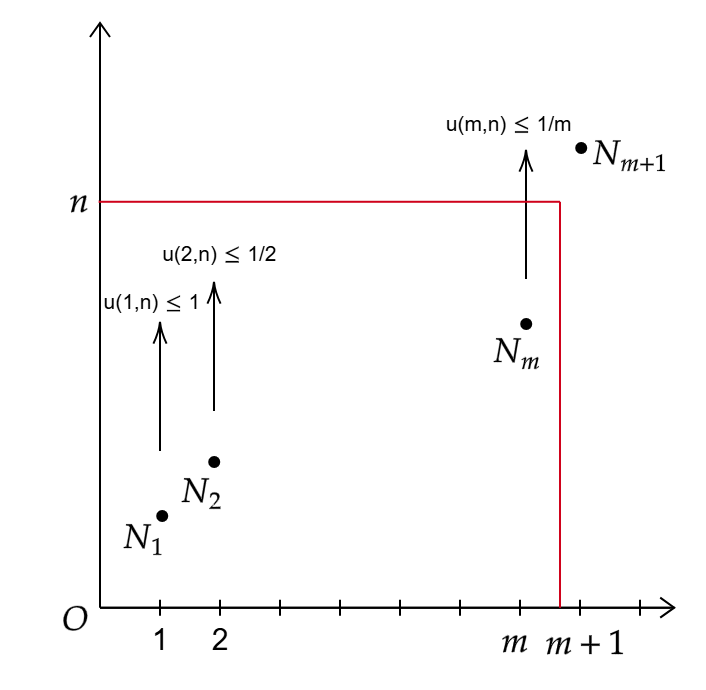
\includegraphics[width=0.58\textwidth]{figures/03-diagonal-sequence.png}
  \caption{对角序列 $m_n$ 的构造示意图（Mathcha 绘制）}
  \label{fig:ch3:diagonal-sequence}
\end{figure}

\end{proof}

下面证明定理~\ref{thm:ch3:3-11}。

\begin{proof}

不失一般性，我们让每个 $X_{nj}$ 的均值 $\mu_{nj}=0$ ，且每行方差和 $\sigma_n^2=1$ ，不然的话可用 $\frac{X_{nj}-\mu_{nj}}{\sigma_{n}}$ 代替 $X_{nj}$ 。

\textbf{\emph((2.) $\Rightarrow$ (1.) )}

由引理~\ref{lem:ch3:3-9}，无穷小条件自动成立，我们只需证明 $S_n\overset{\rm d}\to \mathcal N(0,1)$ 。

这里要用到``截断''的思想，取定 $0<\eta<1$ ，记\[ X_{nj}':=\begin{cases} X_{nj},&\text{ 若 }|X_{nj}|\le \eta\\ 0,&\text{ 其它 } \end{cases} \]

并记 $S_n':=\sum_{j=1}^{k_n}X_{nj}'$ 、 $\sigma'^2_n=\sum_{j=1}^{k_n}\mathrm{Var}[X_{nj}']=\mathrm{Var}[S_n']$ 。且由于 $\mathbb{E}[X_{nj}]=0$ ，截断后的随机变量的期望满足
\[\begin{aligned} &\mathbb{E}[X_{nj}']=\int_{|x|\le \eta}x\mathrm{d}F_{nj}(x)=-\int_{|x|> \eta}x\mathrm{d}F_{nj}(x)\\ \implies &|\mathbb{E}[X_{nj}']| = \left| \int_{|x| \le  \eta} x {\rm d}F_{nj}(x) \right| = \left| \int_{|x| > \eta} x {\rm d}F_{nj}(x) \right| \le \frac{1}{\eta} \int_{|x|>\eta} x^2 {\rm d}F_{nj}(x)  \end{aligned}\]
从而，根据 Lindeberg 条件，

\begin{equation}
\label{eq:ch3:tag-7}
|\mathbb{E}[S_n']| \le \sum_{i=1}^{k_n} |\mathbb{E}[X_{nj}']| \le \frac{1}{\eta} \sum_{j=1}^{k_n} \int_{|x| > \eta} x^2  {\rm d}F_{nj}(x) \to 0
\end{equation}

类似地，我们考虑 $X'^2_{nj}$ 时，由于 $\sigma_n^2=1$ ，
\[\sum_{i=1}^{k_n} \mathbb{E}[X'^2_{nj}] = \sum_{j=1}^{k_n} \int_{|x|\le \eta} x^2 \mathrm{d}F_{nj}(x) =\underbrace{ \sum_{j=1}^{k_n}  \int_{\mathbb R} x^2 {\rm d}F_{nj}(x)}_{\displaystyle =\sigma_n^2=1} - \underbrace{\sum_{j=1}^{k_n} \int_{|x|\geq \eta} x^2 {\rm d}F_{nj}(x)}_{\substack{\text{ 由 Lindeberg 条件 }\\ \displaystyle \to 0}}\to 1\]
同时由式~\eqref{eq:ch3:tag-7}，
\[
\sum_{j=1}^{k_n}(\mathbb{E}[X'_{nj}])^2\le \left(\sum_{j=1}^{k_n}|\mathbb{E}[X_{nj'}]|\right)^2\to0.
\]

我们得出
\[\sigma'^2_n = \mathrm{Var}[S'_n]= \underbrace{\sum_{j=1}^{k_n} \mathbb{E}[X'^2_{nj}] }_{\displaystyle \to 1}- \underbrace{\sum_{j=1}^{k_n} (\mathbb{E}[X'_{nj}])^2 }_{\displaystyle \to 0}\to 1\]
总结一下，前面的分析告诉我们 $\mathbb{E}[S_n']\to 0$ 而 $\sigma'^2_n\to 1$ ，从而， $\frac{\mathbb{E}[S_n']}{\sigma_n'}\to 0$ 。根据
\[
\frac{S_n'}{\sigma_n'}=\frac{S_n'-\mathbb{E}[S_n']}{\sigma_n'}+\frac{\mathbb{E}[S_n']}{\sigma_n'},
\]

$\frac{S_n'}{\sigma_n'}$ 和 $\frac{S_n'-\mathbb{E}[S_n']}{\sigma_n'}$ 应有相同的极限分布。

下一步证明 $\frac{S_n' - \mathbb{E}[S_n']}{\sigma_n'} \overset{\rm d}\to \mathcal{N}(0, 1)$ 。根据 Lindeberg 条件，对任意的 $m\ge 1$ ，

$$\lim_{n\to\infty}m^2\sum_{j=1}^{k_n}\int_{|x|>1/m}x^2{\rm d}F_{nj}(x)=0$$

因此由引理~\ref{lem:ch3:3-12}，存在一列 $\{m_n\}$ 单调递增趋向于 $\infty$ ，使得 

$$\lim_{n\to\infty}m_n^2\sum_{j=1}^{k_n}\int_{|x|>1/m_n}x^2{\rm d}F_{nj}(x)=0$$

如果记 $\eta_n:=m_n^{-1}$ ，并用 $\eta_n$ 替代 $|X'_{nj}|$ 定义中的 $\eta$ ，那么

$$|X_{nj}'|\le \eta_n\quad \text{ 且 }\quad \lim_{n\to\infty}\eta_n=0$$

根据推论~\ref{cor:ch3:3-2}，立即有 $\frac{S_n'-\mathbb{E}[S_n']}{\sigma'_n}\overset{\rm d}\to\mathcal N(0,1)$ ，从而，根据刚刚的分析， 同样有 $\frac{S_n'}{\sigma'_n}\overset{\rm d}\to \mathcal{N}(0,1)$ 。再结合 $\sigma_n'\to 1$ ，我们便得到了 $S_n'\overset{\rm d}\to \mathcal N(0,1)$ 。

回顾一下，我们欲证目标是``未截断''的 $S_n\overset{\rm d}\to \mathcal N(0,1)$ ，既得``已截断''的情形 $S_n'\overset{\rm d}\to \mathcal N(0,1)$ ，根据 Slutsky 定理，只需再表明 $S_n-S_n'\overset{P}\to 0$ 。而这也是容易的， 因为
\[ P(S_n\neq S_n')\leq P\left(\bigcup_{j = 1}^{k_n}\{X_{nj}\neq X_{nj}'\}\right)\leq \sum_{j = 1}^{k_n}P(|X_{nj}|\geq \eta_n) \leq \sum_{j = 1}^{k_n}\frac{1}{\eta_n^2}\int_{|x| > \eta_n}x^2 {\rm d}F_{nj}(x) \to 0 \]

如所欲证。

\textbf{\emph((1.) $\Rightarrow$ (2.))}

令 $\phi_{nj}$ 是 $X_{nj}$ 的特征函数， (1.) $S_{n} \overset{\rm d}\to \mathcal N(0,1)$ 告诉我们，对任意的 $t\in\mathbb R$ ，
\[\lim_{n\to \infty}\prod_{j = 1}^{k_n}\phi_{nj}(t) = e^{-t^2 / 2},\quad \lim_{n\to \infty}\sum_{j = 1}^{k_n}\log \phi_{nj}(t) = -\frac{t^2}{2}\]
根据引理~\ref{lem:ch3:3-8}，(2.) 无穷小条件告诉我们，
\[\lim_{n\to \infty} \max_{1\leq j\leq k_n}|\phi_{nj}(t) - 1| = 0\]
按照引理~\ref{lem:ch3:3-3} 证明中相同的论证（赋 $\theta_{nj} = \phi_{nj}(t) - 1$ ），可知以下等式成立，

\begin{equation}
\label{eq:ch3:tag-9}
\log \phi_{nj}(t)  = \phi_{nj}(t) - 1 + \lambda_{nj}|\phi_{nj}(t) - 1|^{2}
\end{equation}

其中 $|\lambda_{nj}| < 1$ 。

根据 Taylor 展开，对某个 $|\xi_t|\le 1$ ，
\[\sum_{j = 1}^{k_n}|\phi_{nj}(t) - 1| = \sum_{j = 1}^{k_n}\left|\int_{\mathbb R} (e^{itx} - 1){\rm d}F_{nj}(x)\right| =\sum_{j = 1}^{k_n}\left|\int_{\mathbb R} \left(itx + \xi_t\frac{t^2x^2}{2}\right){\rm d}F_{nj}(x)\right|\leq \frac{t^2}{2}\int_{\mathbb R}x^2\mathrm{d}F_{nj}(x)= \frac{t^2}{2} < \infty\]
因此

\begin{equation}
\label{eq:ch3:tag-8}
\sum_{j = 1}^{k_n}|\phi_{nj}(t) - 1|^2\leq \max_{1\leq j\leq k_n}|\phi_{nj}(t) - 1|\sum_{j = 1}^{k_n}|\phi_{nj}(t) - 1| \to 0
\end{equation}

即，式~\eqref{eq:ch3:tag-9} 进行求和并取极限后，第二项是可忽略的，结合式~\eqref{eq:ch3:tag-8} 便有了：
\[\lim_{n\to \infty} \sum_{j=1}^{k_n} (\phi_{nj}(t) - 1) = \lim_{n\to \infty} \sum_{j=1}^{k_n} \log \phi_{nj}(t) = -\frac{t^2}{2}\]
把实部摘出来：
\[\lim_{n\to \infty} \sum_{j=1}^{k_n} \int_{-\infty}^{\infty} (1 - \cos tx) {\rm d}F_{nj}(x) = \frac{t^2}{2}\]
我们将积分区域分为 $|x|\le \eta$ 和 $|x|>\eta$ 两部分， $\eta>0$ ，则上式告诉我们，对任意 $\epsilon>0$ ，存在充分大的 $n$ 有
\[\begin{aligned} \frac{t^2}{2} - \sum_{j=1}^{k_n}\int_{|x|\le\eta}(1-\cos tx){\rm d}F_{nj}(x) &\le \sum_{j=1}^{k_n}\int_{|x|>\eta}(1-\cos tx){\rm d}F_{nj}(x) + \epsilon\\ &\le 2\sum_{j=1}^{k_n} P(|X_{nj}|>\eta) + \epsilon\\ &\le \frac{2}{\eta^2} + \epsilon\qquad \text{\scriptsize Chebyshev} \end{aligned}\]
另一方面，利用 $1-\cos tx \le \frac{t^2 x^2}{2}$ 还可得到
\[\begin{aligned} \frac{t^2}{2} - \sum_{j=1}^{k_n}\int_{|x|\le\eta}(1-\cos tx){\rm d}F_{nj}(x) &\ge  \frac{t^2}{2} -  \frac{t^2}{2}\sum_{j=1}^{k_n}\int_{|x|\le \eta}x^2{\rm d}F_{nj}(x) \\ &=\frac {t^2}2\sum_{j=1}^{k_n}\int_{|x|>\eta}x^2{\rm d}F_{nj}(x) \qquad {\scriptstyle \sigma_n^2=1}\\  \end{aligned}\]
将上面的两式结合，我们最终得到了 (在 $n$ 充分大时)，
\[\sum_{j=1}^{k_n}\int_{|x|>\eta}x^2\mathrm{d}F_{nj}(x)\leq \frac{4}{t^2 \eta^2} + \frac{2 \epsilon}{t^2}\]
令 $t \to \infty$ ，我们便证明了 Lindeberg 条件。

\end{proof}

Lindeberg-Feller CLT（定理~\ref{thm:ch3:3-11}）的充分性（(2.) $\Rightarrow$ (1.)）由 Lindeberg 于 1922 年证明，必要性（(1.) $\Rightarrow$ (2.)）由 Feller 于 1935 年证明。这个定理是概率论中影响最为深远的成果之一。几乎所有各种类型中心极限定理的推广都源于 Lindeberg-Feller 中心极限定理。

\subsection{例子：回归}

有如下线性回归模型：
\[
y_{j} = x_{j}\beta +\epsilon_{j},\quad j=1,2,3,\dots.
\]

其中误差项 $\epsilon_j$i.i.d. 服从均值为 0、方差为 $\sigma_\epsilon^2$ 的分布；$x_j$ 是固定的常数，也称作设计点 (design point) ，满足 

$$\max_{1\leq j\leq n}\frac{|x_j|}{a_n}\to 0,\quad\text{ 其中 } a_n^2 := \sum_{j = 1}^n x_j^2$$

这个条件直观上意味着没有任何一个 $x_j$ 可以主导回归系数的估计。

普通最小二乘 (OLS) 估计量如下：
\[\widehat{\beta}_{LS} = \frac{\sum_j x_j y_j}{\sum_j x_j^2} = \frac{\sum_j x_j (x_j \beta + \epsilon_j)}{a_n^2} = \beta + \frac{\sum_j x_j \epsilon_j}{a_n^2}\]
这个估计量有多好？它的渐近分布如何呢？ 我们将上式写作 \[ a_n(\widehat{\beta}_{LS} - \beta) = \sum_{j=1}^n \left( \frac{x_j}{a_n} \epsilon_j \right) \]并注意到，若将 $X_{nj} = \frac{x_j \epsilon_j}{a_n}$ 视作三角组列 $\{X_{nj}:1\le j\le n\}_{n\ge 1}$ 的元素，则其满足

\begin{itemize}
\tightlist
\item
  $\mu_{nj}=\mathbb E[X_{nj} ]= 0$ ；
\item
  $\sigma_{nj}^2 = \text{Var}[X_{nj}] = \frac{x_j^2}{a_n^2} \sigma_\epsilon^2$ ；
\item
  $\sigma_n^2 = \sum_{j=1}^n \sigma_{nj}^2 = \frac{\sum_j x_j^2}{a_n^2} \sigma_\epsilon^2 = \sigma_\epsilon^2$ 。
\end{itemize}

我们可以直接验证 Lindeberg 条件成立：记 $m_n:=\max\limits_{j=1,\dots, n}\left|\frac{x_j}{a_n}\right|$ ，那么 $m_n\to 0$ ，有
\[\begin{aligned} \frac1{\sigma_n^2}\sum_{j = 1}^{n}\int_{|x|>\delta\sigma_n}x^2{\rm d}F_{nj}(x)&= \frac{1}{\sigma_n^2a_n^2}\sum_{j = 1}^{n}x_j^2\int_{|x\epsilon_j / a_n| > \delta \sigma_n} \epsilon_j^2{\rm d}F_{\epsilon_j}(x) \qquad \text{\scriptsize 代入}{\scriptstyle X_{nj}=\tfrac{x_j\epsilon_j}{a_n}} \\ &\le \frac1{\sigma_\epsilon^2a_n^2}\sum_{j = 1}^{n}x_j^2\int_{|\epsilon_j|>\delta\sigma_\epsilon/m_n}\epsilon_j^2{\rm d}F_{\epsilon_j}(x)\\ &=\frac1{\sigma_\epsilon^2}\int_{|\epsilon_j|>\delta\sigma_\epsilon/m_n}\epsilon_j^2{\rm d}F_{\epsilon_j}(x)\qquad \text{\scriptsize 由}{\scriptstyle \epsilon_j}\text{\scriptsize i.i.d.}\\ &\to 0,\text{ 当 }n\to\infty \end{aligned}\]
最后一行来自控制收敛定理：
\[
\lim\limits_{n\to\infty}\mathbb{E}[\epsilon_j^2\mathbb I(|\epsilon_j|>\delta\sigma_\epsilon/m_n)]=\mathbb{E}\Big[\lim\limits_{n\to\infty}\epsilon_j^2\mathbb{I}(|\epsilon_j|>\delta\sigma_\epsilon/m_n)\Big]=0.
\]
由定理~\ref{thm:ch3:3-11}，
\[
a_n(\widehat{\beta}_{LS} - \beta) = \sum_{j = 1}^{n}X_{nj}\overset{\rm d}\to \mathcal N(0,\sigma_\epsilon^2).
\]

\section{相依随机变量的中心极限定理}

关于非独立情况，概率论学者讨论得较多且获得实际应用的有相依随机变量序列、强平稳随机变量序列、鞅、马尔可夫过程及其他泛函，以及各种类型的统计量序列。对于这些序列在附加一定条件时，中心极限定理也成立。这便使得许多实际问题中的随机变量或随机过程可视为正态的。

我们这里介绍一种一种比较简单的情形，作为 Lindeberg-Feller 定理的简单推广。

\begin{definition*}[$m$-相依]

若一列随机变量 $\{X_n\}_{n=1}^\infty$ 满足：存在正整数 $m$ ，使得对任意 $j-i> m$ ，有 $(X_1,X_2,\dots,X_i)$ 与 $(X_{j},X_{j+1},\dots,X_n)$ (生成的 $\sigma$ 域) 总独立，则称这列随机变量是 \textbf{\emph{$m$-相依}} (m-dependent) 的。

\end{definition*}

\begin{remark}
对固定随机变量序列，上述定义中的 $m$ 是固定的；在三角阵列等随样本量变化的设定中，也可另行考虑 $m=m_n$ 随 $n$ 变化的情形，有些文献称之为 $f(n)$-相依。
\end{remark}

$m$-相依序列广泛出现在时间序列分析中，如滑动平均（Moving Average, MA）模型。下面的定理说明，在合适的条件下，中心极限定理对这类序列仍然成立。

\begin{theorem}

\label{thm:ch3:3-13}

设有一列 $m$ -相依的随机变量 $\{X_n\}_{n=1}^\infty$ ，记 $S_n:=\sum\limits_{j=1}^nX_j$ 、 $\sigma_n^2:=\mathrm{Var}[S_n]$，若如下条件成立：

\begin{enumerate}
\def\labelenumi{\arabic{enumi}.}
\tightlist
\item
  一致有界，即，存在常数 $M$ 使得 $\sup_n|X_n|\le M$ ；
\item
  当 $n\to\infty$ 时， $\frac{\sigma_n}{mn^{1/3}}\to \infty$ ；
\item
  $m=o(n^{1/3})$ ；
\end{enumerate}

那么，
\[
\frac{S_n-\mathbb{E}[S_n]}{\sigma_n}\overset{\rm d}\to \mathcal N(0,1).
\]

\end{theorem}

\begin{proof}

不失一般性设均值 $\mathbb {E}[X_j]=0$ 。总的思路是使用``分块''技术：将 $n$ 个变量分为 $p$ 个大块和 $p$ 个小块：

\begin{itemize}
\tightlist
\item
  \emph{大块}：大小通常远大于 $m$ ，这里取 $k = [n^{1/3}]$ ，块内随机变量的和记作 $Y_i,\,i=1,\dots,p$ 。
\item
  \emph{小块}：大小为 $m$ ，块内随机变量的和记作 $Z_i,i=\,1,\dots,p$ 。
\end{itemize}

每类块的数量为 $p=\left[\frac n{k+m}\right]=O(n^{2/3})$ 。分块布局是下面这种``大块连着小块''的样子：
\[\underbrace{X_1 ,\dots, X_k}_{\text{大块 }},\; \underbrace{X_{k+1}, \dots ,X_{k+m}}_{\text{小块 }},\; \underbrace{X_{k+m+1} ,\dots, X_{2k+m}}_{\text{大块 }},\; \underbrace{X_{2k+m+1}, \dots, X_{2k+2m}}_{\text{小块 }},\dots\]
从而求和可写作
\[
\begin{aligned}
S_n={}&\underbrace{(X_1+ \cdots+ X_k)}_{Y_1} + \underbrace{(X_{k+1}+ \dots +X_{k+m})}_{Z_1}\\
&+ \underbrace{(X_{k+m+1} +\dots +X_{2k+m})}_{Y_2}+ \underbrace{(X_{2k+m+1}+ \dots +X_{2k+2m})}_{Z_2}\\
&+ \dots + \text{余项 } R_p.
\end{aligned}
\]
其中 $R_p:=X_{p(k+m)}+\cdots+X_n$ 。记全体大块之和为 $S'_n:=\sum\limits_{i=1}^pY_i$ 、小块之和为 $S_n'':=\sum\limits_{i=1}^{p}Z_i$ 、余项之和为 $S_n'''=R_p$ ，这便将全体和分成了三部分：
\[
S_n=S'_n+S_n''+S_n'''.
\]

分块的好处在于，``小块''充当了``阻挡依赖性''的作用： $Y_1,Y_2,\dots,Y_p$ 两两之间至少相隔了 $m$ ，因而是相互独立的。由于当 $n$ 足够大时 $k\gg m$ ，因而 $Z_i$ 之间也同样独立。

接下来我们表明大块负责贡献了正态性：具体来说，大块之和 $S_n'$ 满足 CLT，而小块和 $S_n''$ 及残余项 $S_n'''$ 则可忽略。

\begin{itemize}
\tightlist
\item
  小块：由一致有界性，每个小块的方差 $\mathrm{Var}[Z_i]\le m^2M^2$ ；由 $Z_i$ 两两独立性知所有小块的方差之和 $\mathrm{Var}[S_n'']=\sum_{i=1}^p\mathrm{Var}[Z_i]\le pm^2M^2=O(n^{2/3}m^2)$ 。于是 $S_n''=O_P(\sqrt{\mathrm{Var}[S_n'']})=O_P(n^{1/3}m)$ 。
\item
  余项：余项长度小于 $k+m$ ，由一致有界性可知这部分 $|S_n'''|\le (k+m) M$； 即 $S_n'''=O_P(k+m) = O_P(n^{1/3})$。
\end{itemize}

由条件 $\frac{\sigma_n}{mn^{1/3}}\to\infty$，显然小块部分和余项都满足 $\frac{S_n''}{\sigma_n}\overset{P}\to 0$、$\frac{S_n'''}{\sigma_n}\overset{P}\to 0$。

下面来处理大块。我们构造三角组列： $\{Y_j:1\le j\le n\}_{n\ge 1}$ ，记 $\sigma'^2_n:=\mathrm{Var}[S_n']$ ，由 $|Y_n|\le kM$ 可知

$$\max_{1\le j\le n} \left|\frac{Y_j}{\sigma_n'}\right|\le \frac{kM}{\sigma_n'}$$

为了应用推论~\ref{cor:ch3:3-2}（这个一致有界条件蕴含了 Lyapunov 条件和 Lindeberg 条件），我们希望当 $n\to\infty$ 时上式能 $\to 0$；或者，将 $k=[n^{1/3}]$ 代入，我们希望能证明 $\sigma_n'/n^{1/3}\to\infty$ 。

回顾一下，定理的条件告诉我们 $\frac{\sigma_n}{mn^{1/3}}\to\infty$ ，只要能证明 $\sigma'_n\sim \sigma_n$ 是同阶的，不就证出来了吗？

自此到达最后一步：证明 $\sigma'_n\sim \sigma_n$ 。这一步比较繁琐。由
\[\begin{aligned}\mathbb{E}[S^2_n] = \mathbb{E}[S'^2_n] + \mathbb{E}[S''^2_n] + \mathbb{E}[S'''^2_n] + 2\mathbb{E}[S'_n S''_n] + 2\mathbb{E}[S''_n S'''_n] + 2\mathbb{E}[S'''_n S'_n]\\ \end{aligned}\]
有\[\begin{aligned}
|\mathbb{E}[S^2_n] - \mathbb{E}[S'^2_n]|
&\leq |\mathbb{E}[S''^2_n] + \mathbb{E}[S'''^2_n] + 2\mathbb{E}[S'_n S''_n] + 2\mathbb{E}[S''_n S'''_n] + 2\mathbb{E}[S'''_n S'_n]|\\
&\leq p m^2 M^2 + (k + m)^2 M^2 + 4p(mM)^2 + 2m(k + m)M^2.
\end{aligned}\]这里我们用到了 $\mathbb{E}[S'_n S''_n] = \sum_{j,l=1}^p \mathbb{cov}(Y_j, Z_l) =\sum_{j=1}^p \big(\mathbb{cov}(Y_j, Z_j) + \mathbb{cov}(Y_j, Z_{j-1})\big) \leq 2p(mM)^2$（利用 $m$ 相依导致大部分协方差为 0）。类似地 $\mathbb{E}[S''_n S'''_n] \leq 2m(k + m)M^2$ 以及 $\mathbb{E}[S'''_n S'_n] = \mathrm{Cov}[S'''_n, S'_n] = 0$ 。

因此， 

\[
1 - \frac{\sigma'^2_n}{\sigma^2_n}
\leq \frac{6pm^2M^2 + 2(k + m)^2M^2 + 2m(k + m)M^2}{\sigma_n^2}
=O\left(\frac{m^2n^{2/3}}{\sigma_n^2}\right)\longrightarrow 0.
\]

故 $\frac{\sigma_n'^2}{\sigma_n^2}\to 1$，我们完成了证明。

\end{proof}
最后整理一下证明过程：

\begin{enumerate}
\def\labelenumi{\arabic{enumi}.}
\tightlist
\item
  我们首先对 $X_1,\dots,X_n$ 进行分块，用长为 $m$ 的小块 $Z_i$ 来隔离大块 $Y_i$ ；
\item
  证明小块和余项加起来是 $o_P(1)$ 的，Slutsky 定理告诉我们这俩不影响极限分布；
\item
  对独立的大块序列 $Y_i$ 用 Lindeberg-Feller CLT（定理~\ref{thm:ch3:3-11}），而 Lindeberg 条件成立当 $\sigma_n'/n^{1/3}\to\infty$ 。
\item
  最后表明 $\sigma'^2_n/\sigma_n^2\to 1$ ，结合定理给出的条件，可知上一步的 Lindeberg 条件确实成立。
\end{enumerate}


\begin{remark}

\begin{itemize}
\tightlist
\item
  这个``分块''方案叫做 \textbf{\emph{Bernstein Blocking Method}} 。
\item
  如果去掉``一致有界''的假设，能否证明相依序列的 CLT 呢？答案是肯定的，请参阅 \cite{janson2021}。
\end{itemize}
\end{remark}
